\subsection{Sensitivity to quadratic pitch damping}
\label{sec:nonlinear-pitch}

The largest linear-model registration gain occurs near pitch resonance, where high angular speed also amplifies rate-dependent damping. Suzuki et al. fitted linear and quadratic pitch damping to free-decay tests on a floating wind turbine platform \cite{Suzuki2021Floater}. We adopt the form of that damping law for a sensitivity study with prescribed coefficients. The pitch equation retains the original wave-slope excitation and adds a damping torque proportional to angular speed squared. After dividing by the effective pitch inertia, it becomes
\begin{equation}
  \ddot\theta+d_1\dot\theta+d_2|\dot\theta|\dot\theta+\omega_n^2\theta
  =-\omega_n^2 G\,\partial_x\eta(\mathbf{0},t),
  \label{eq:quadratic-pitch}
\end{equation}
where $d_1=2\zeta\omega_n$. The two damping terms dissipate mechanical power per unit effective inertia at the rate $d_1\dot\theta^2+d_2|\dot\theta|^3$. To prescribe the strength of the nonlinear term, we use $\chi=d_2 v_{\mathrm{ref}}/d_1$, the ratio of quadratic to linear damping torque magnitudes at $v_{\mathrm{ref}}=0.123$ rad/s, the peak pitch rate of the linear mode at the reference wave. We test $\chi=0$, $0.25$, $0.50$, and $1.00$, spanning the linear baseline through equal damping contributions at that speed.

We integrate Eq.~\eqref{eq:quadratic-pitch} directly from rest and use the cycle following 60 forcing periods to evaluate the phase-shifted pitch at every spoke and midpoint. The new pitch changes both the pointing angle and the rotated antenna lever arm, so we recompute the diffraction path and mapping at each visit. We pair the same incident waves, roll, surge, and heave across damping levels, with 192 visits in each of 32 initial phases. At $\chi=0$, direct integration reproduces the acquisition and registration decisions of the closed-form solution in all seven tested wave conditions. Extending spin-up to 80 cycles and halving the maximum integration step changes pitch by at most $6.6\times10^{-12}$ rad and leaves every visit classification identical. Cycle-integrated forcing work balances dissipation and the change in mechanical energy to a relative residual below $4.4\times10^{-14}$.

\begin{figure*}[t]
\centering
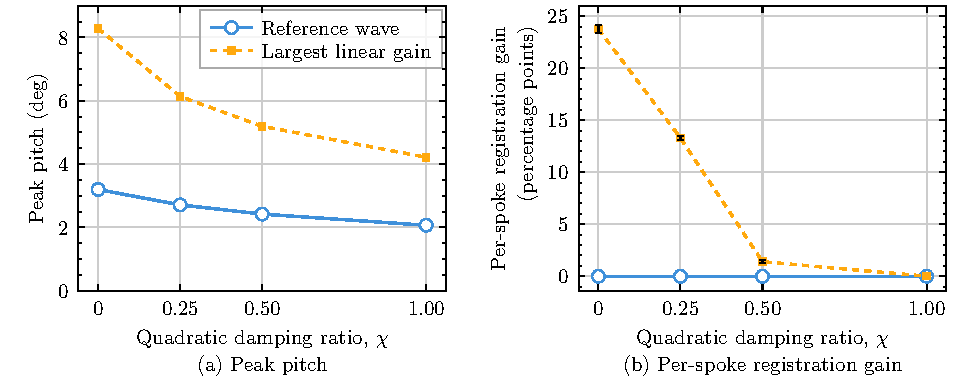
\includegraphics[width=.95\textwidth]{figures/operating/nonlinear-pitch.pdf}
\caption{Peak pitch and registration gain as the quadratic pitch damping increases. The reference wave is 0.350 Hz and 0.150 m. The largest-gain cell of the linear map is 0.3325 Hz and 0.432 m. Gain measures the increase in usable visits over midpoint registration. Error bars give paired 95\% intervals over initial wave phases.}
\label{fig:nonlinear-pitch}
\end{figure*}

At the largest-gain cell, the quadratic term dissipates 51.4\% of the cycle's input work at $\chi=1$. The fundamental pitch lag rises from $71.1^\circ$ to $81.0^\circ$ and the third harmonic reaches 0.81\% of the fundamental amplitude. As peak pitch falls from $8.28^\circ$ to $4.21^\circ$, the scan-midpoint estimate satisfies the position tolerance for progressively more of the acquired echoes. Figure~\ref{fig:nonlinear-pitch} shows the per-spoke registration gain falling from 23.76 to 13.30 to 1.40 to 0.00 percentage points, even as body-pointed acquisition rises from 38.05\% to 38.57\%. The 0.30375 Hz neighbor at fixed amplitude, the 0.376 m neighbor at fixed frequency, and the pilot wave all reach zero registration gain at $\chi=0.25$.

At the reference wave, all acquired echoes meet the position tolerance throughout the damping sweep. Lower pitch increases body-pointed acquisition from 92.97\% to 95.31\% and reduces the additional gain from leveling by $2.34\pm1.72$ percentage points at $\chi=1$ relative to $\chi=0$, using the paired phase interval. The neighboring 0.345 and 0.355 Hz waves also retain zero registration gain at the reference amplitude. These cases show that near resonance, the damping law affects whether midpoint registration crosses the position tolerance, while wave obstruction still limits acquisition in the larger-amplitude conditions.
